\scanpage{23}
\reversemarginpar
\margin{\handwritten{SGA 4 $\overline{\text{\uline{VI}}}$ 2}}
\normalmarginpar

\uline{Exercice} \handwritten{2}. . Soi\inserted{en}t $C$ une \deleted{\unsure{\uline{U}-|\uline{U}}}\inserted{petite} catégorie\handwritten{,}\inserted{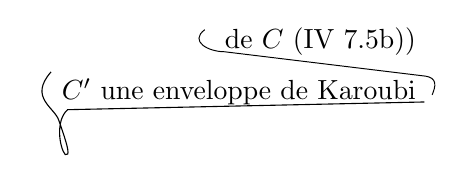
\begin{tikzpicture}[baseline=(kar.base),x=1cm,y=1cm]
\node[inner sep=0pt,anchor=base west] (kar) at (0,0) {$C'$ une enveloppe de Karoubi};
\node[inner sep=0pt,anchor=base east] (ref) at ([yshift=.55cm]kar.east) {\inserted{de $C$ (IV 7.5\handwritten{b))}}};
\draw[line width=.4pt] (-.13,.35) .. controls (-.42,.02) and (-.08,-.10) .. (-.03,-.27)
 .. controls (.10,-.64) and (.11,-.72) .. (.05,-.70)
 .. controls (-.02,-.62) and (-.08,-.27) .. (.08,-.13)
 -- ([xshift=.10cm,yshift=-.13cm]kar.east);
\draw[line width=.35pt] ([xshift=-.25cm,yshift=.15cm]ref.west)
 .. controls ([xshift=-.45cm]ref.west) and ([xshift=-.20cm,yshift=-.13cm]ref.west)
 .. ([yshift=-.13cm]ref.west)
 -- ([xshift=.10cm,yshift=.20cm]kar.east)
 .. controls ([xshift=.28cm,yshift=.18cm]kar.east) and ([xshift=.24cm,yshift=.06cm]kar.east)
 .. ([xshift=.20cm,yshift=-.04cm]kar.east);
\end{tikzpicture}} Montrer que les conditions suivantes sont équivalentes:

(i) La catégorie $\mathrm{Ind}(C)$ (I 8.2) est un \uline{$U$}-topos.

( bis) Le foncteur canonique $\mathrm{Ind}(C)\handwritten{\longrightarrow}\overset{\handwritten{\scriptscriptstyle\wedge}}{C}$ admet un adjoint à droite qui \deleted{commute aux} e\unsure{\deleted{n}s|\deleted{s}n}t ex\(\mathbb{a}\)ct à gauche.

(i ter) Il existe une topologie sur $C$ pour laquelle les faisceaux soient les préfaisceaux ind-représentables.

\figure{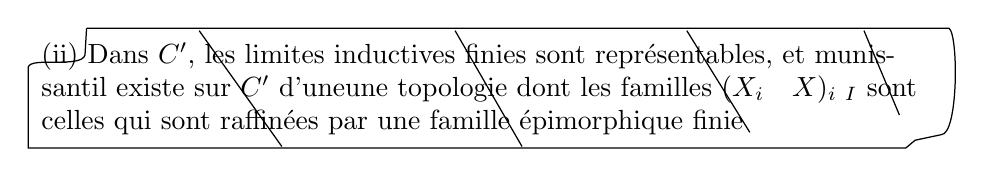
\begin{tikzpicture}
\node[inner sep=4pt,anchor=north west,text width=.94\linewidth] (oldii) at (0,0)
{\deleted{(ii) Dans $C'$, les limites inductives finies sont représentables, \deleted{et munissant}\inserted{il existe sur} $C'$ \deleted{\unsure{d'une}}\inserted{une} topologie dont les familles $(X_i\quad X)_{i\ I}$ sont celles qui sont raffinées par une famille épimorphique finie}};
\draw[line width=.45pt] ([xshift=.72cm,yshift=.03cm]oldii.north west)
 -- ([xshift=-.02cm,yshift=.03cm]oldii.north east)
 .. controls ([xshift=.10cm,yshift=-.05cm]oldii.north east)
 and ([xshift=.10cm,yshift=.15cm]oldii.south east)
 .. ([xshift=-.12cm,yshift=.15cm]oldii.south east)
 -- ([xshift=-.45cm,yshift=.08cm]oldii.south east)
 -- ([xshift=-.57cm,yshift=-.02cm]oldii.south east)
 -- ([xshift=-.02cm,yshift=-.02cm]oldii.south west)
 -- ([xshift=-.02cm,yshift=-.46cm]oldii.north west)
 .. controls ([xshift=.02cm,yshift=-.33cm]oldii.north west)
 and ([xshift=.65cm,yshift=-.48cm]oldii.north west)
 .. ([xshift=.70cm,yshift=-.31cm]oldii.north west)
 -- ([xshift=.72cm,yshift=.03cm]oldii.north west);
\draw[line width=.45pt] ([xshift=2.15cm]oldii.north west)--([xshift=3.20cm]oldii.south west);
\draw[line width=.45pt] ([xshift=5.40cm]oldii.north west)--([xshift=6.25cm]oldii.south west);
\draw[line width=.45pt] ([xshift=-3.35cm]oldii.north east)--([xshift=-2.55cm,yshift=.18cm]oldii.south east);
\draw[line width=.45pt] ([xshift=-1.10cm]oldii.north east)--([xshift=-.65cm,yshift=.40cm]oldii.south east);
\end{tikzpicture}}

(ii) \deleted{Dans $C'$} I\begin{tikzpicture}[baseline=(ell.base),x=1em,y=1ex]
\node[inner sep=0pt,anchor=base] (ell) at (0,0) {l};
\draw[line width=.45pt] (-.19,2.05)--(.19,2.05)--(.19,2.35);
\draw[line width=.45pt] (-.19,-.40)--(.02,-.40)--(.02,-.72);
\end{tikzpicture} existe une topologie sur $C'$ dont les familles couv\unsure{\deleted{a}r|\deleted{r}a}a\unsure{\deleted{t}n|\deleted{n}t}tes sont celles qui so\unsure{\deleted{j}n|\deleted{n}j}t raffinées par une famille épimorphique (ou encore, épimorphique effective universelle ..) \uline{finie}, dans $C'$ les limites \deleted{projectives}\inserted{inductives} finies sont représentables, et le foncteur canonique $C\handwritten{\longrightarrow}\overset{\handwritten{\scriptscriptstyle\sim}}{C}$ \deleted{est} y commute.

(iii) (Si dans $C$ les limites projectives finies sont représentab\deleted{\unsure{l|e}}les,\deleted{\unsure{â|à}} de sorte qu'on peut prendre $C'=C$.) Dans $C$ les limites inductives finies sont représentables, et $C$ satisfait la condition ST) de
\reversemarginpar\margin{\handwritten{$\times$}}\normalmarginpar
I 8.8 f).

(iv) Il existe un topos $E$ engendré par sa sous-catégorie pleine
\reversemarginpar\margin{\handwritten{$\times$}}\normalmarginpar
$E_{\mathrm{PF}}$ (\quad\quad), et une équivalence de catégories $C'\handwritten{\approxeq}E_{\mathrm{PF}}$.

De plus, \deleted{la topologie} si ces conditions sont satisfaites, la topologie postulée dans (i ter) est nécessairement celle décrite dans (ii), et le topos $E$ postulé dans (iv) est nécessairement équivalent à $\mathrm{Ind}(C)$. Ce topos est donc parfait si et seulement si \inserted{dans} $C'$ \deleted{est} les limites projectives finies sont r\unsure{\deleted{r}e|\deleted{e}r}présentables.
% archive sheet number: 22

